\documentclass{article}

\usepackage{standalone}
\usepackage{pgfplots}
\pgfplotsset{compat=newest}
\usepackage{tikz}
\usetikzlibrary{decorations.markings}
\usetikzlibrary{patterns}

\usepackage{subcaption}
\usepackage[margin=2.5cm]{geometry}
\usepackage{amsmath}
\usepackage{amssymb}


\newcommand\greybox[1]{
	\vskip\baselineskip
	\par\noindent\colorbox{lightgray}{
		\begin{minipage}{\textwidth}#1\end{minipage}
	}
	\vskip\baselineskip
}

\title{En-dimensionale potensialer}


\begin{document}
\maketitle


Vi skal i dette kapitelet se på en rekke forskjellige en-dimensionale potensialer, som vi løser
S.L. for og finner bølgefunksjonene til, og ser på tolkninger av.

\section{Partikkel i brønn}
Vi skal nå se på en partikkel som befinner seg i en potensial-brønn. Dette er beskrevet av 
potensialet 
\begin{align}
	 V(x) = \begin{cases}
		0 \hspace{0.75cm} |x| < \frac{a}{2} \\
		V_0 \hspace{.625cm} |x| \ge \frac{a}{2} 
		\end{cases}
\end{align}
Dette ligner partikkel i boks scenarioet vi så tidligere, men her er ikke potensialet uendelig 
stort utenfor boksen, slik at partikkelen kan befinne seg der også.

\begin{figure}[h!]
     \centering
     \begin{subfigure}[b]{0.4\linewidth}
       \centering
	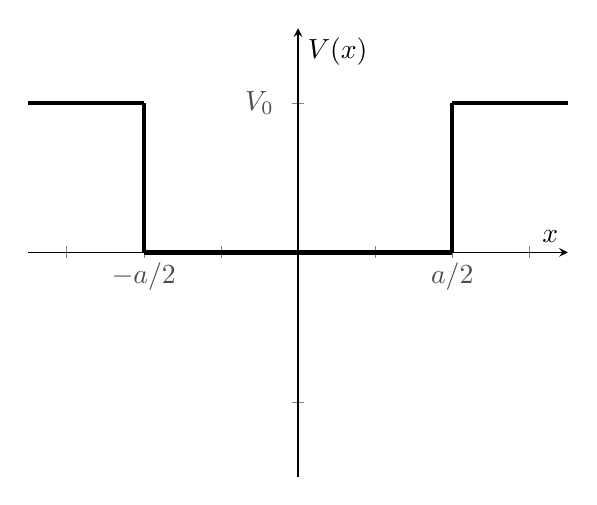
\begin{tikzpicture}
	  \begin{axis}%
	    [
	     xlabel=$x$,
	     ylabel=$V(x)$,
	     axis lines=middle,
	     restrict y to domain=-1:2.,
	     enlargelimits={abs=.75},
	     yticklabels=\empty,
	     xticklabels=\empty
	    ]
	    \addplot+[mark=none, 
		    domain=-1:1,
		    samples=150,
		    draw=black!70,
		    pattern color=black,
	    	    area legend] { 0 }  ;
	    \node [color=black!70] at (-0.25, 0.5) {$V_0$};
	    \node [color=black!70] at (1, -0.08) {$a /2$};
	    \node [color=black!70] at (-1, -0.08) {$-a /2$};
	\draw [ultra thick] (1, 0.5) -- (2,0.5);
	\draw [ultra thick] (-1, 0.5) -- (-2,0.5);
	\draw [ultra thick] (1, 0) -- (1,0.5);
	\draw [ultra thick] (-1, 0) -- (-1,0.5);
	\draw [ultra thick] (-1, 0) -- (1,0);
	  \end{axis}
	\end{tikzpicture}
         \label{fig:cos}
     \end{subfigure}
       \caption{Potensialet $V(x)$ til partikkel-brønn.}
        \label{fig:bølger}
\end{figure}
Vi løser nå S.L. for dette potensialet ved å dele opp problemet i flere områder.
Vi ser på løsningene for $|x|<a /2$, $x>a/2$ og $x<-a /2$ hver for seg og 
bruker randbetingelser for å fuge de sammen til en koherent bølgefunksjon. 
Vi skal også begrense oss til å se på bølgefunksjoner som har energi mindre enn $V_0$.
For hver av de tre tilfellene får vi essensielt en fri-partikkel S.L. som vi må løse.
Vi minner oss på at vi har den tidsuavhengige S.L. som
\begin{align}
	 \frac{-\hbar^2}{2m} \frac{\partial^2 \psi}{\partial x^2} + V(x)\psi  = E\psi
\end{align}
Vi starter med $|x|<a$, hvor vi har 
\begin{align}
	 \frac{\partial^2 \psi}{\partial x^2}  = -k^2\psi
\end{align}
hvor $k=\sqrt{2mE} /\hbar$. Her kjenner vi de elementære løsningene  
\begin{align}
	 \psi = Ae^{ikx} + B e^{-ikx}
\end{align}
For $|x|>a / 2$ har vi 
\begin{align}
	 \frac{\partial^2 \psi}{\partial x^2}  = \kappa^2\psi
\end{align}
hvor vi nå har $\kappa = \sqrt{2m(V_0-E)}/\hbar$. Vi husker at vi antok $E<V_0$ og vi får da 
den generelle løsningene på høyre og venstre siden for brønnen 
\begin{align}
	 \psi = Ce^{\kappa x} + D e^{-\kappa x}
\end{align}
Vi bruker nå randbetingelser og at vi vil ha en fysikalsk, dvs. normaliserbar, bølgefunksjon.
Vi må derfor ha at $\psi \to 0$ når $|x|\to\infty$, hvilket fører til at vi har 
\begin{align}
	 \psi &= Ce^{\kappa x} \hspace{0.75cm} x < \frac{a}{2} \\
	 \psi &= D e^{-\kappa x} \hspace{0.6cm} x > \frac{a}{2}
\end{align}
Vi må nå fuge sammen bølgefunksjonene i de tre regionene ved å bruke kravet om at bølgefunksjonene 
og deres deriverte skal være kontinuerlige. Siden om dette ikke er tilfellet så eksisterer
strengt talt ikke den andre-deriverte og da er det vanskelig å gi mening til S.L.
Vi krever derfor at bølgefunksjonene i de forskjellige regionene er like i $\pm a / 2$.
\begin{align}
	 Ce^{-\kappa\frac{a}{2}} &= Ae^{-ik \frac{a}{2}} + B e^{ik \frac{a}{2}} \label{eq:mina}\\
	 De^{-\kappa\frac{a}{2}} &= Ae^{ik \frac{a}{2}} + B e^{-ik \frac{a}{2}} \label{eq:maxa}
\end{align}
og tilsvarende for de deriverte av bølgefunksjonen 
\begin{align}
 \kappa Ce^{-\kappa\frac{a}{2}} &= ik(Ae^{-ik \frac{a}{2}} - B e^{ik \frac{a}{2}}) \label{eq:dmina}\\
 -\kappa De^{-\kappa\frac{a}{2}} &= ik(Ae^{ik \frac{a}{2}} - B e^{-ik \frac{a}{2}}) \label{eq:dmaxa}
\end{align}
Vi dividerer \ref{eq:mina} på \ref{eq:dmina} for å eliminere $C$.
\begin{align}
 \frac{ik}{\kappa} 
&= \frac{Ae^{-ik \frac{a}{2}} + B e^{ik \frac{a}{2}}}{Ae^{-ik \frac{a}{2}} - B 
e^{ik \frac{a}{2}}}  \label{eq:AB_1_start}\\
	\Rightarrow \hspace{0.4cm} ik( Ae^{-ik \frac{a}{2}} - B e^{ik \frac{a}{2}} )
	&= \kappa(Ae^{-ik \frac{a}{2}} + B e^{ik \frac{a}{2}}) \\
	\Rightarrow \hspace{0.4cm} ik Ae^{-ik \frac{a}{2}} - \kappa Ae^{-ik \frac{a}{2}}
	&= ik B e^{ik \frac{a}{2}}  + \kappa B e^{ik \frac{a}{2}} \\
	\Rightarrow \hspace{0.4cm} (ik - \kappa) Ae^{-ik \frac{a}{2}} 
	&= (ik +\kappa)B e^{ik \frac{a}{2}}   \\
\Rightarrow \hspace{0.4cm} \frac{A}{B} &= \frac{ik + \kappa}{ik - \kappa} e^{ik a}  \label{eq:AB_1}
\end{align}
Tilsvarende kan vi dividerer \ref{eq:maxa} på \ref{eq:dmaxa} for å eliminere $D$.
\begin{align}
 \frac{ik}{-\kappa} 
&= \frac{Ae^{ik \frac{a}{2}} + B e^{-ik \frac{a}{2}}}{Ae^{ik \frac{a}{2}} 
- B e^{-ik \frac{a}{2}}}   \label{eq:AB_2_start}  \\
  \Rightarrow \hspace{0.4cm} ik( Ae^{ik \frac{a}{2}} - B e^{-ik \frac{a}{2}} )
 &= -\kappa(Ae^{ik \frac{a}{2}} + B e^{-ik \frac{a}{2}}) \\
	\Rightarrow \hspace{0.4cm} (ik + \kappa)Ae^{ik \frac{a}{2}} 
  &= (ik -\kappa) B e^{-ik \frac{a}{2}} \\
\Rightarrow \hspace{0.4cm}  \frac{A}{B} &= e^{-ik a} \frac{ik -\kappa}{ik + \kappa} \label{eq:AB_2}
\end{align}
Dette gir da når vi multipliserer \ref{eq:AB_1} med \ref{eq:AB_2}
\begin{align}	 
	\big(\frac{A}{B}\big)^2 
	&= e^{-ik a} \frac{ik -\kappa}{ik + \kappa} e^{ik a} \frac{ik +\kappa}{ik - \kappa}\\
	&= 1
\end{align}
Hvilket gir $A=B$ eller $A=-B$.
Vi ser på de to tilfellene hver for seg, og starter med $A=B$ hvor vi umiddelbart ser fra 
\ref{eq:mina} og \ref{eq:maxa} at vi da får $C=D$. Vi har bølgefunksjonen som 
\begin{align}
	 \psi = \begin{cases}
		Ce^{\kappa x} \hspace{1.4cm} x < \frac{a}{2} \\
		2A\cos(kx) \hspace{0.5cm} |x| \le \frac{a}{2} \\
		Ce^{-\kappa x} \hspace{1.2cm} x > \frac{a}{2} \\
		\end{cases}
\end{align}
hvor vi minner os på at Eulers formel gir oss 
\begin{align}
	 \cos(kx) &= \frac{e^{ikx} + e^{-ikx}}{2} \\
	 \sin(kx) &= \frac{e^{ikx} - e^{-ikx}}{2i} 
\end{align}
Vi ser her at bølgefunksjon er symmetrisk $\psi(x) = \psi(-x)$. Videre har vi for $A=B$ at 
\ref{eq:AB_1_start} blir 
\begin{align}
 \frac{ik}{\kappa} 
&= \frac{e^{-ik \frac{a}{2}} + e^{ik \frac{a}{2}}}{e^{-ik \frac{a}{2}} - e^{ik \frac{a}{2}}}\\
&= \frac{\cos(\frac{ka}{2})}{-i\sin(\frac{ka}{2})}
\end{align}
Vi skriver om litt slik at vi har
\begin{align}
	 \tan(\frac{ka}{2}) &= \frac{ \frac{\kappa a}{2} }{ \frac{k a}{2}} \\
  &= \frac{\sqrt{ (\frac{\kappa a}{2}})^2 }{ \frac{ka}{2}} \\
  &= \frac{\sqrt{ \frac{a^2}{4} \frac{2m(V_0-E)}{\hbar^2} } }{ \frac{ka}{2}} \\
  &= \frac{\sqrt{ \frac{a^2}{2} \frac{mV_0}{\hbar^2} 
  	   -(\frac{ka}{2})^2 } }{ \frac{ka}{2}}
\end{align}
Videre definerer vi 
\begin{align}
	 \xi_0 &= \frac{ka}{2} \\ 
	\xi &= \frac{a}{2} \frac{\sqrt{mV_0}}{\hbar}
\end{align}
slik at vi får \ref{eq:AB_1_start} på formen
\begin{align}
	 \tan(\xi) = \frac{\sqrt{\xi_0^2 - \xi^2}}{\xi} \label{eq:trans_s}
\end{align}
Tilsvarende har vi med $A=-B$ at fra \ref{eq:mina} og \ref{eq:maxa} at vi 
må ha $C=-D$. Vi har bølgefunksjonen som 
\begin{align}
	 \psi = \begin{cases}
		Ce^{\kappa x} \hspace{1.4cm} x < \frac{a}{2} \\
		2Ai\sin(kx) \hspace{0.5cm} |x| \le \frac{a}{2} \\
		-Ce^{-\kappa x} \hspace{1.2cm} x > \frac{a}{2} \\
		\end{cases}
\end{align}
hvor vi har brukt Eulers formel slik at vi har 
Vi ser her at bølgefunksjon er asymmetrisk $\psi(x) = -\psi(-x)$. Videre har vi for $A=-B$ at 
\ref{eq:AB_1_start} blir 
\begin{align}
 \frac{-ik}{\kappa} 
= \frac{e^{-ik \frac{a}{2}} - e^{ik \frac{a}{2}}}{e^{-ik \frac{a}{2}} + e^{ik \frac{a}{2}}}
= \frac{i\sin(\frac{ka}{2})}{\cos(\frac{ka}{2})} 
\end{align}
slik at 
\begin{align}
\frac{k}{\kappa} &= -\cot(\frac{ka}{2})
\end{align}
Slik at vi får \ref{eq:AB_1_start} på formen
\begin{align}
	 -\cot(\xi) = \frac{\sqrt{\xi_0^2 - \xi^2}}{\xi} \label{eq:trans_as}
\end{align}
når vi igjen innfører $\xi$ og $\xi_0$.
Lign. \ref{eq:trans_s} og \ref{eq:trans_as} er transcendentale ligninger som vi kan bruke til å 
bestemme energinivåene.



\end{document}

